
%Corps du document :
%\setlength{\parindent}{1cm}    

\section{Conception d'ensemble de l'architecture applicative}

\subsection{Analyse des modèles conceptuels proposés}

\subsection{Établissement des diagrammes de séquences systèmes}

\subsection{Diagrammes d'activité}

\begin {center}
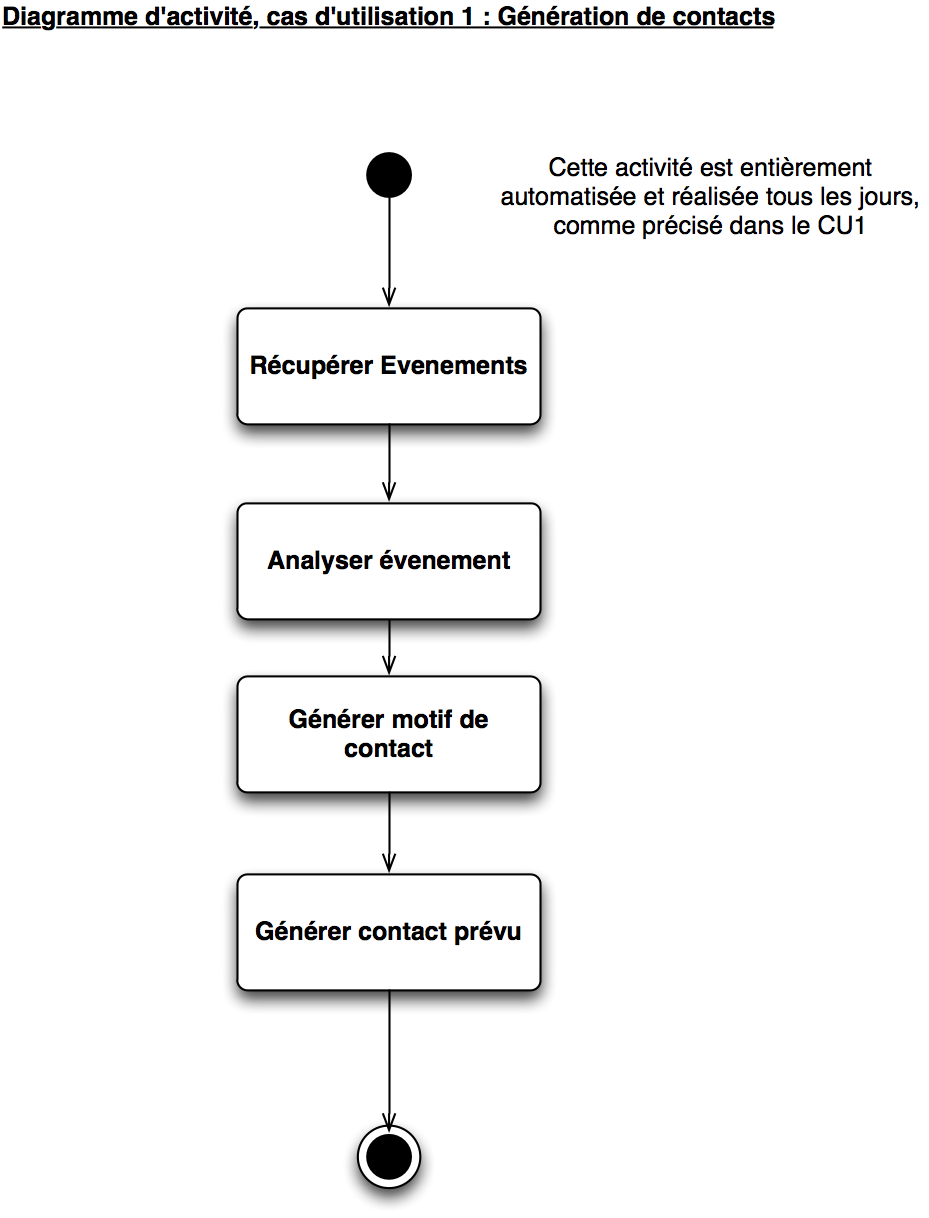
\includegraphics[width=\textwidth]{..\..\diagrammeActivite\DACU1.png}
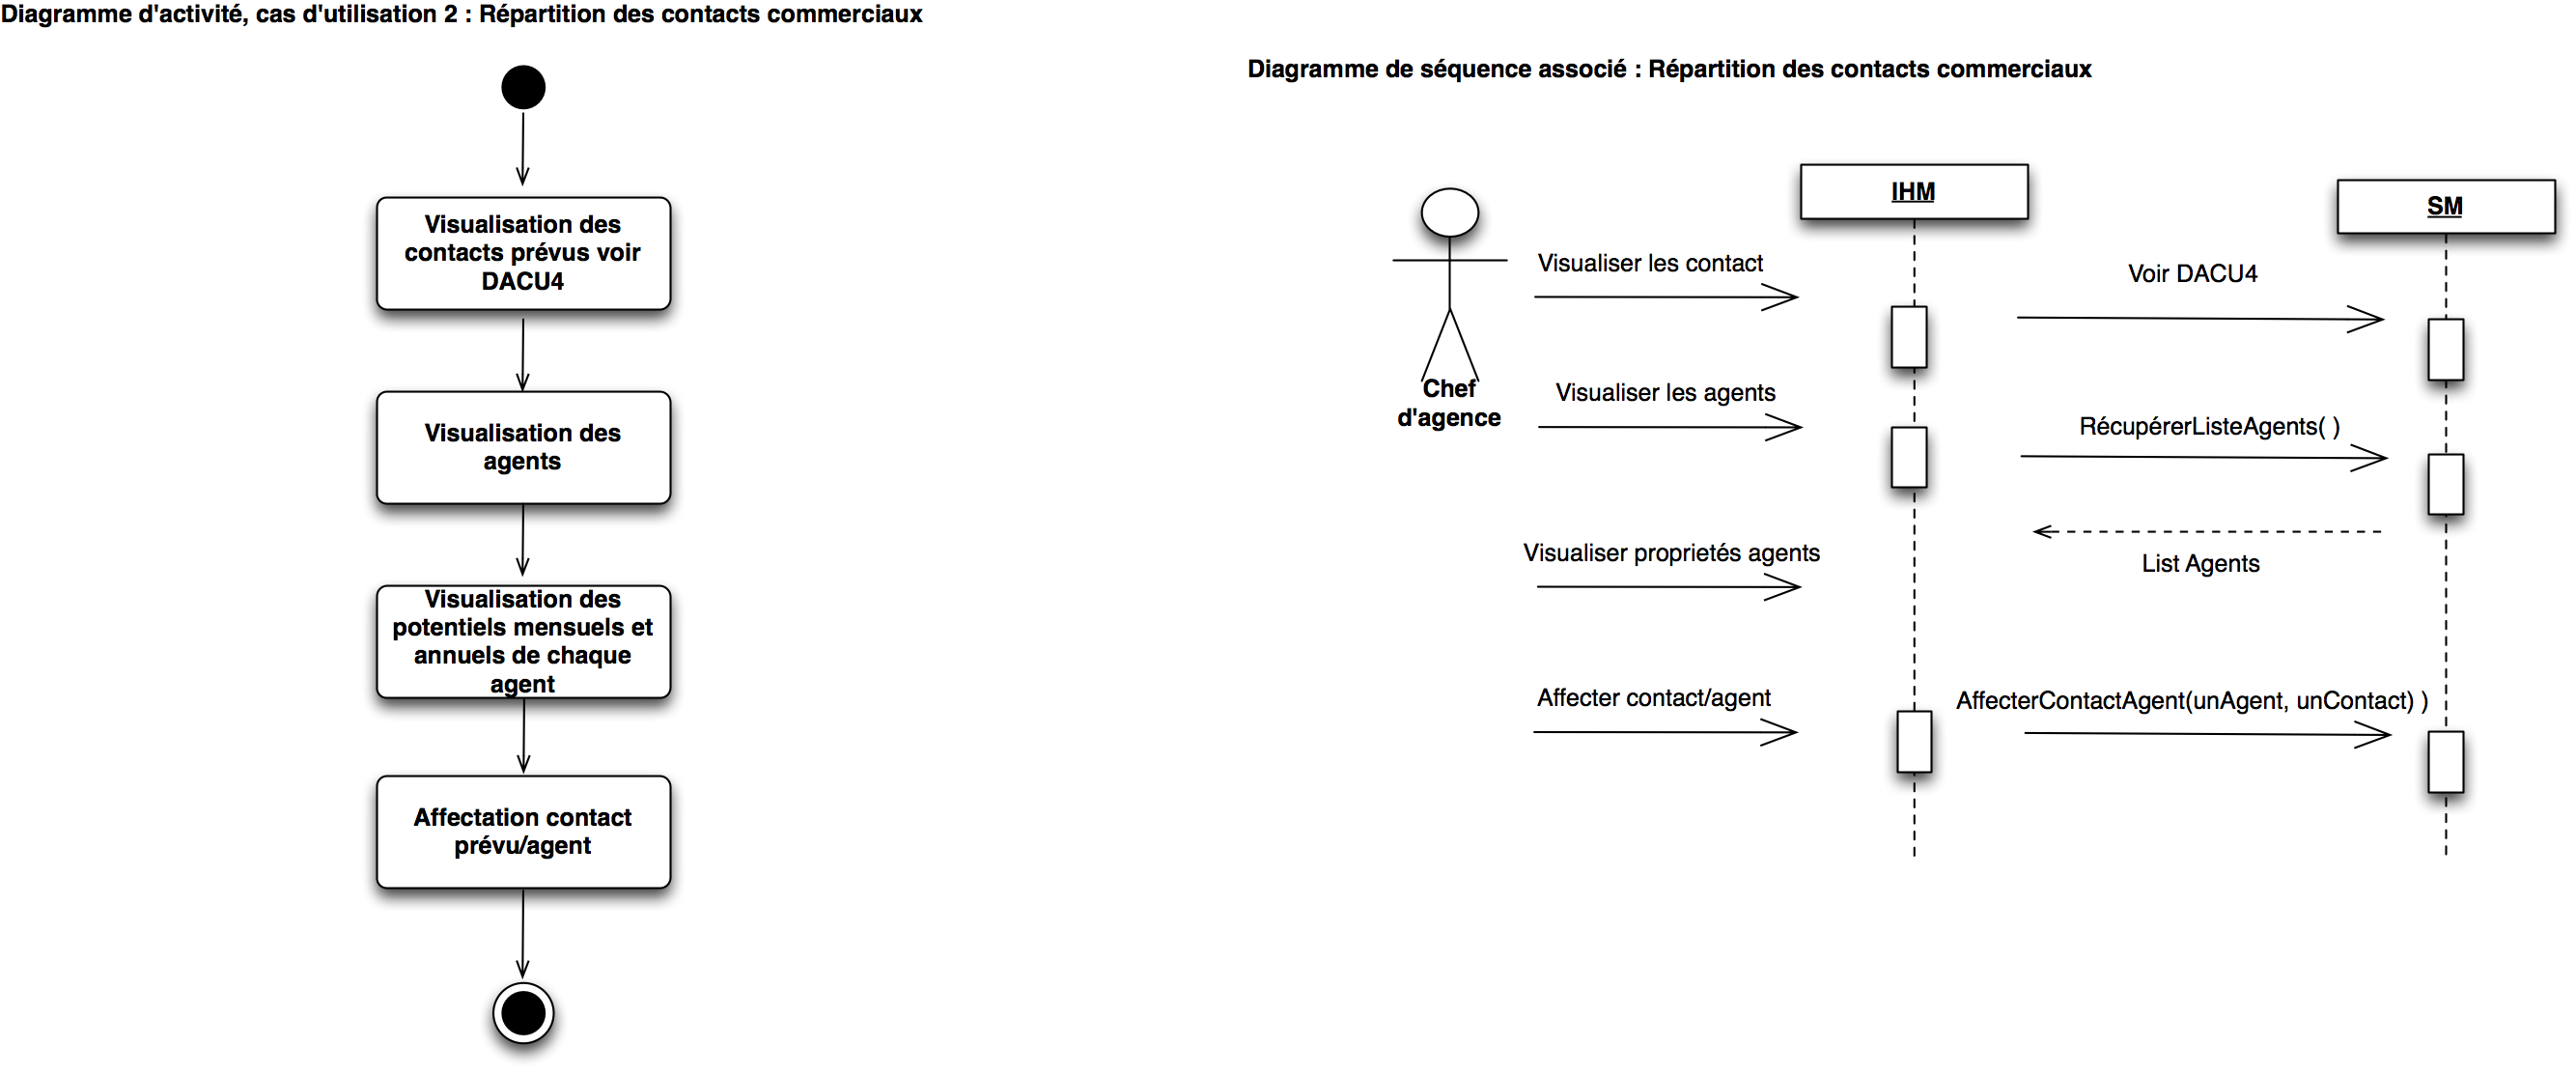
\includegraphics[width=\textwidth]{..\..\diagrammeActivite\DACU2.png}
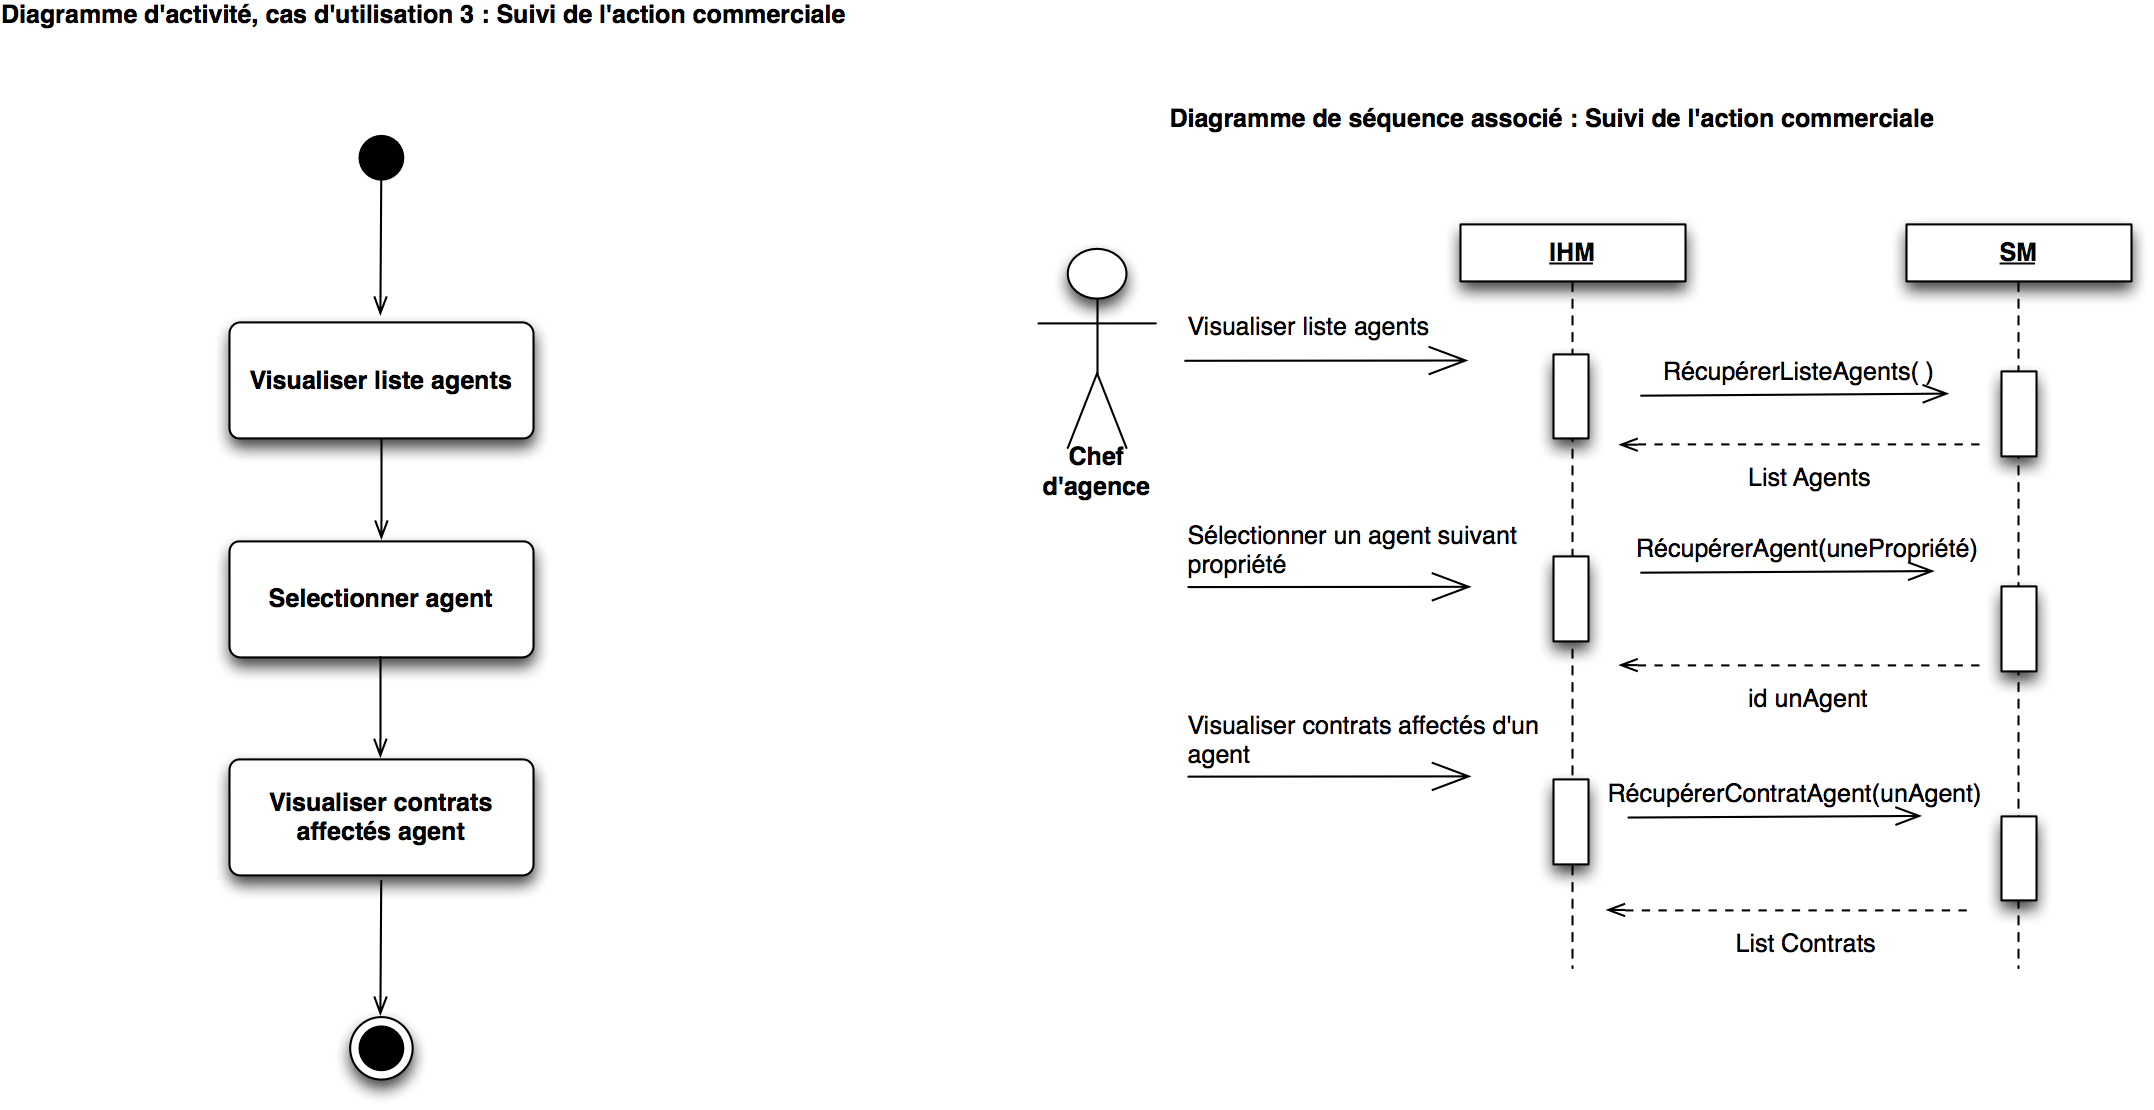
\includegraphics[width=\textwidth]{..\..\diagrammeActivite\DACU3.png}
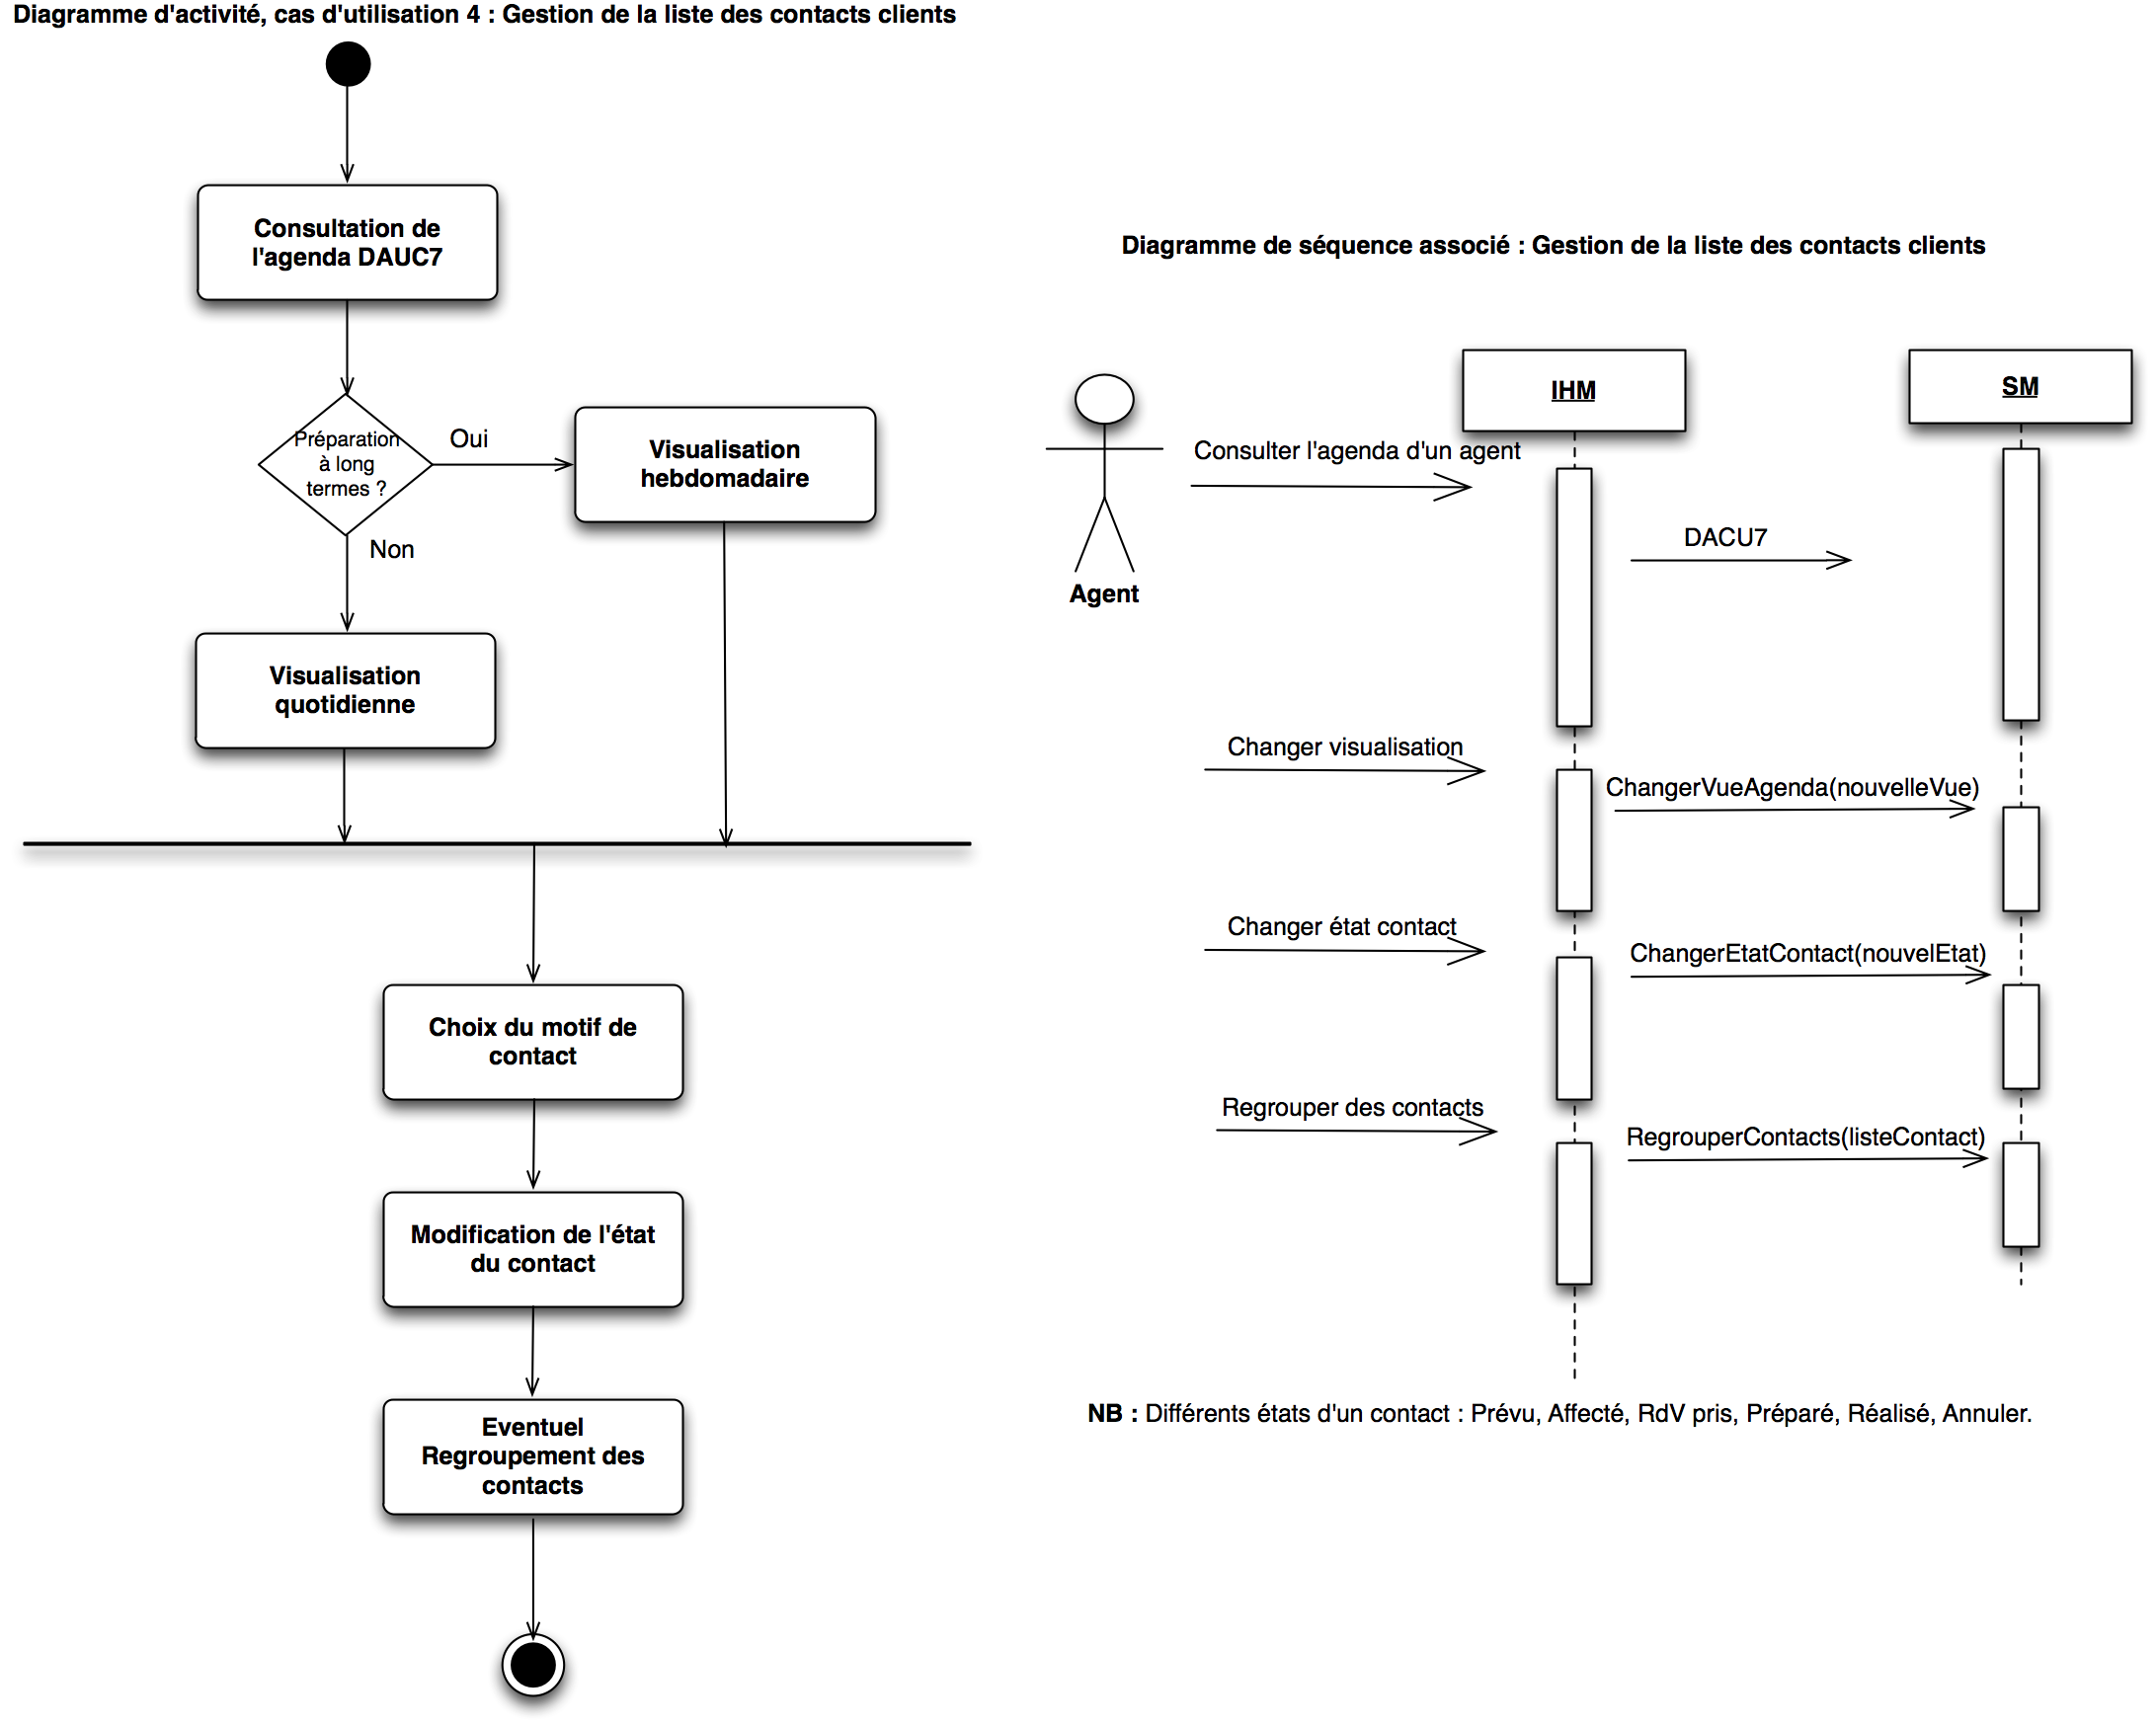
\includegraphics[width=\textwidth]{..\..\diagrammeActivite\DACU4.png}
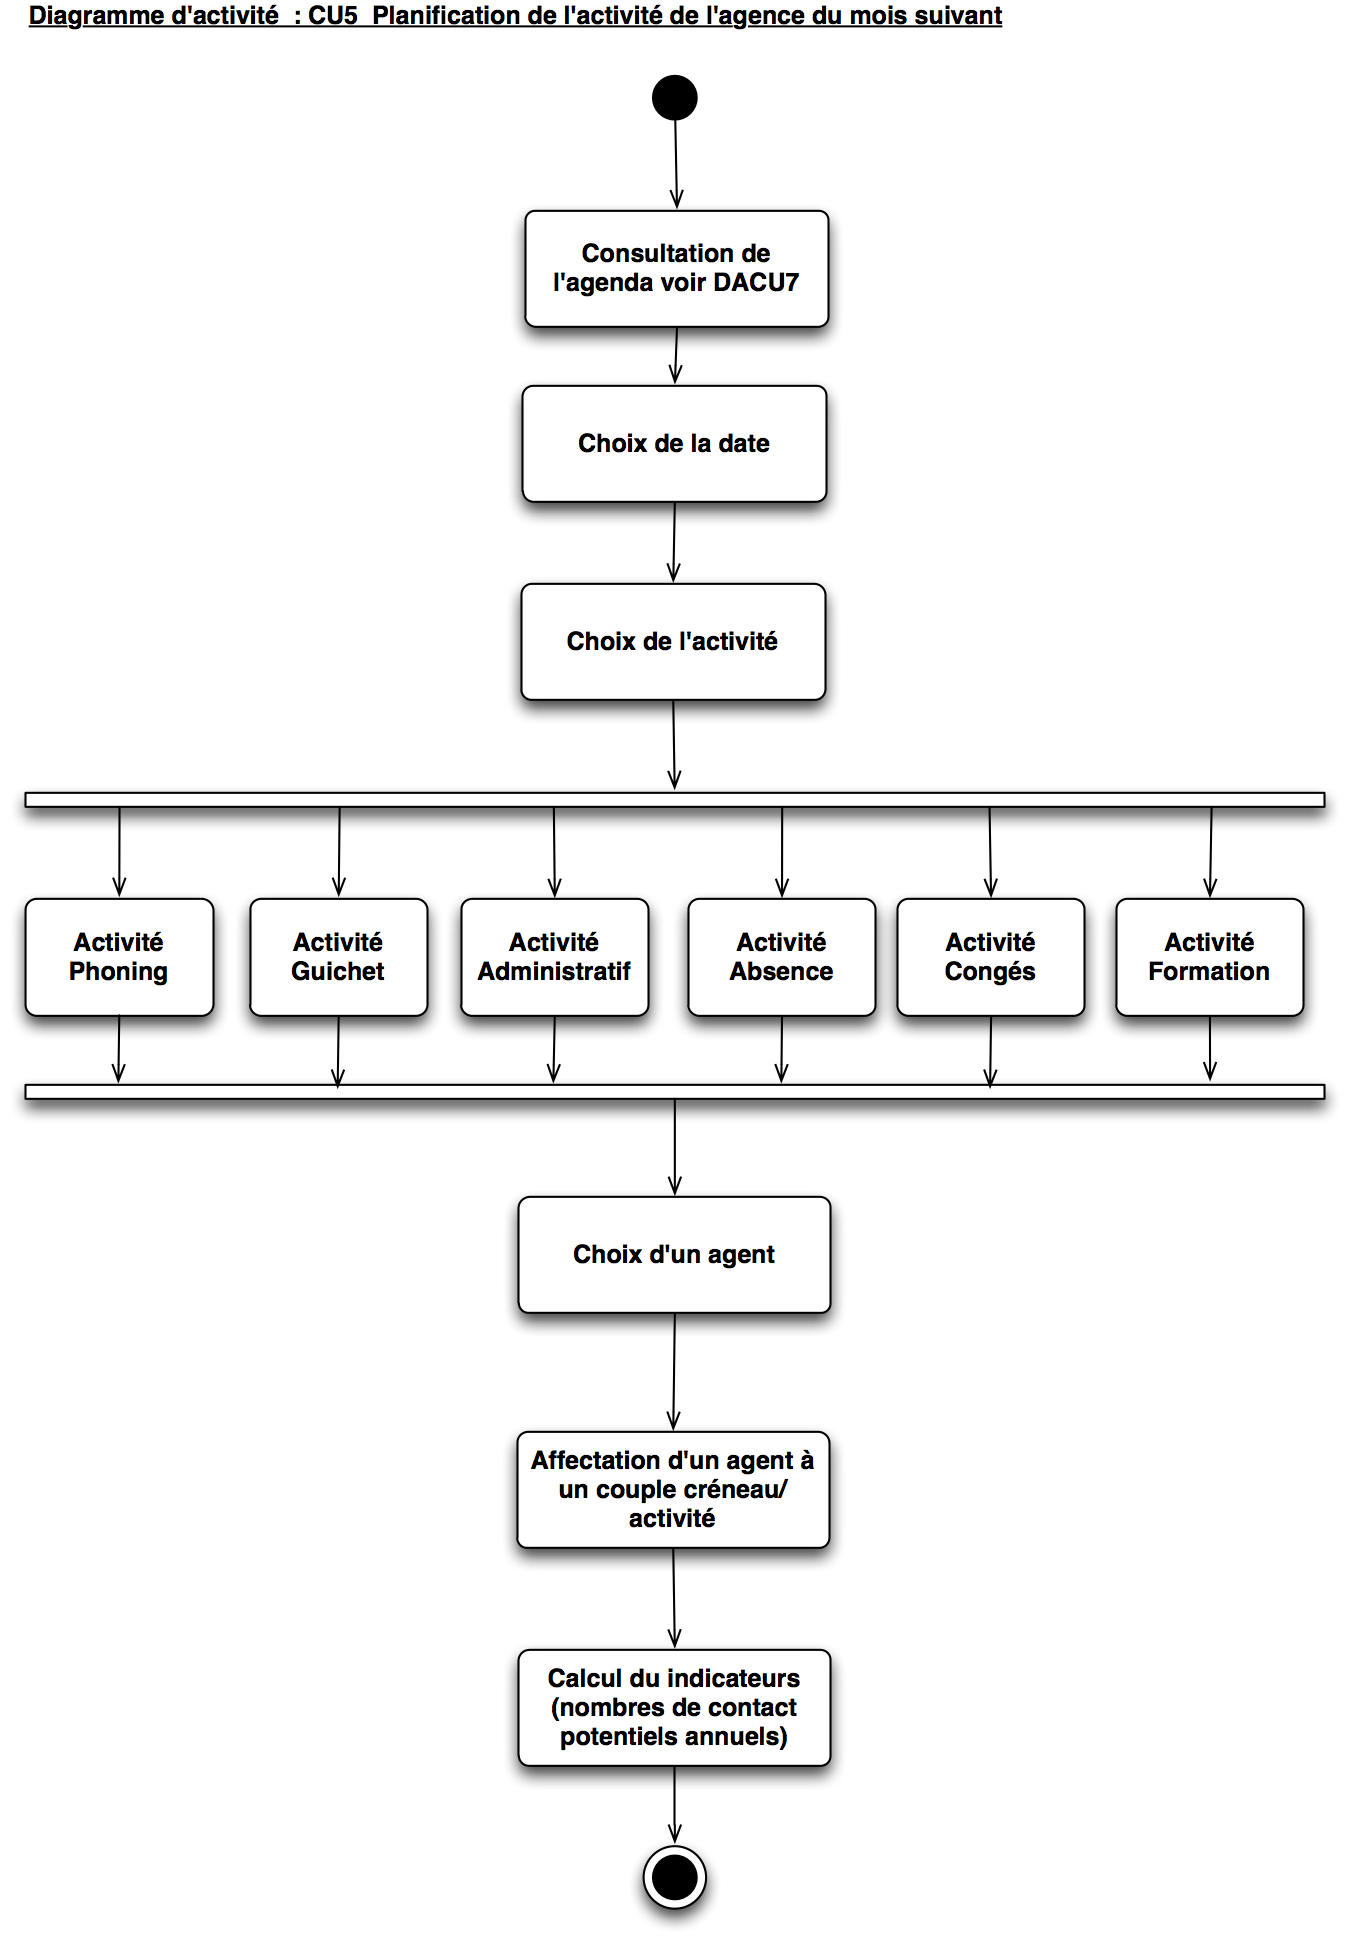
\includegraphics[width=\textwidth]{..\..\diagrammeActivite\DACU5.png}
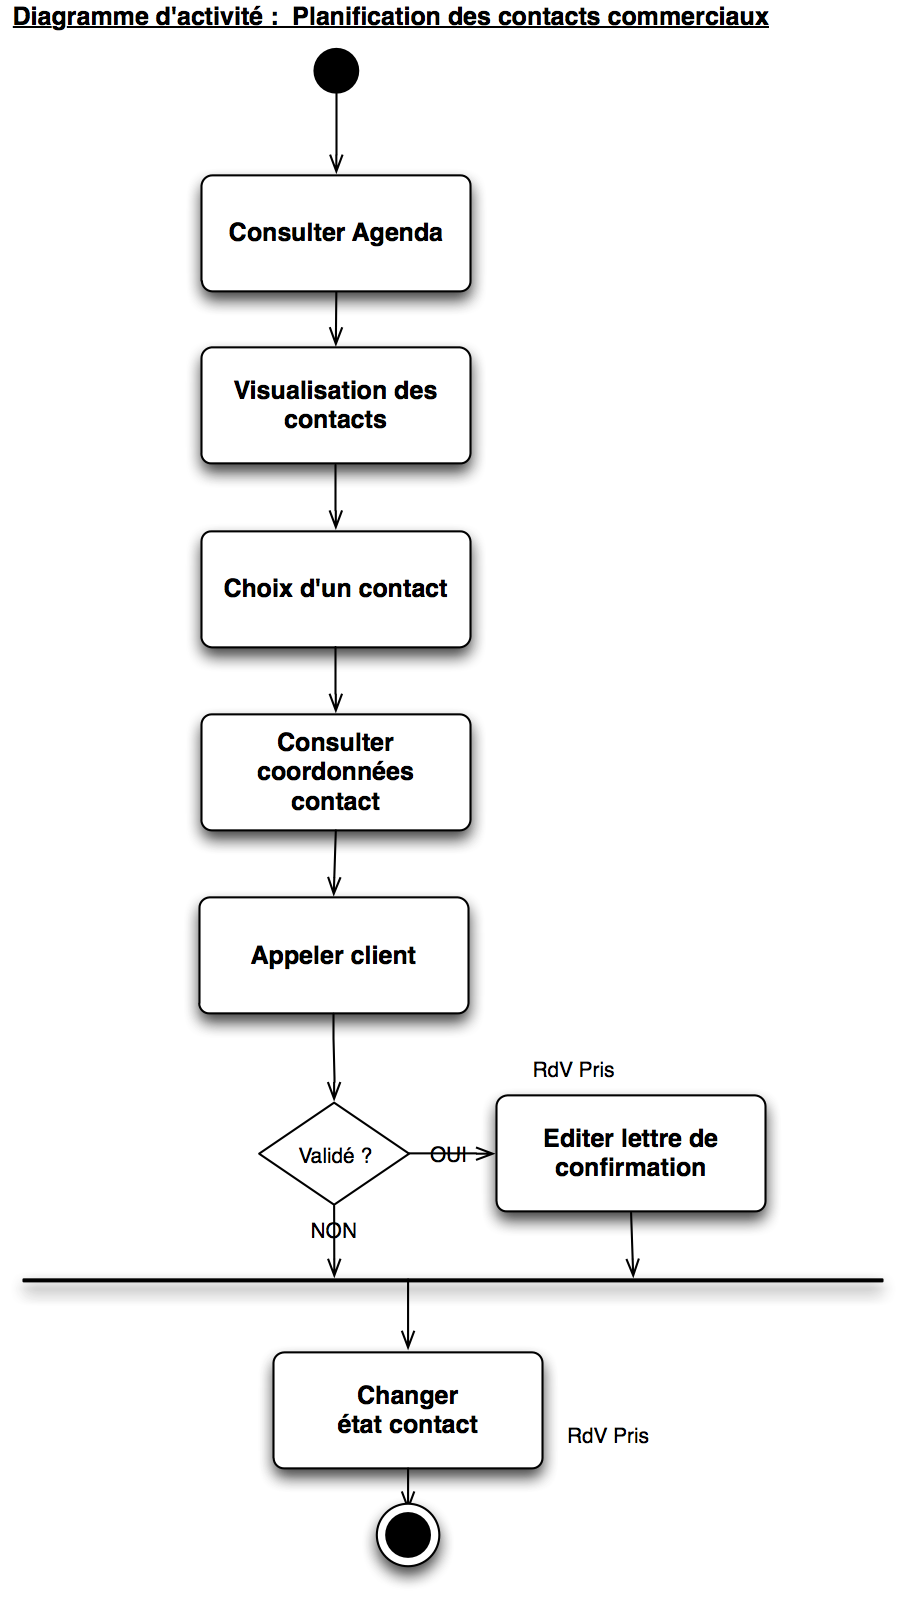
\includegraphics[width=\textwidth]{..\..\diagrammeActivite\DACU6.png}
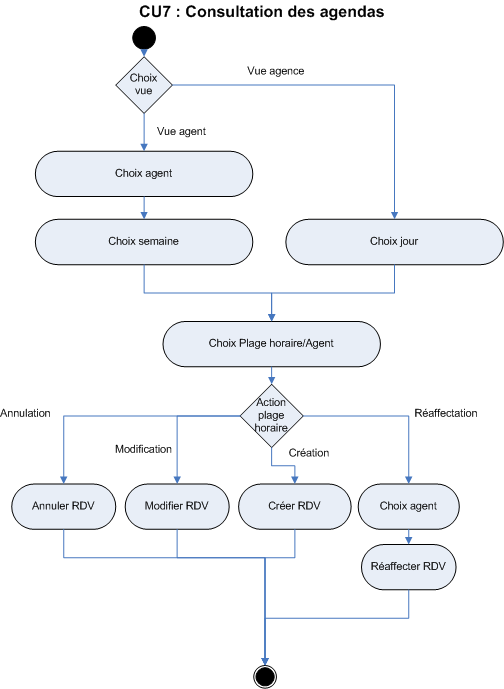
\includegraphics[width=\textwidth]{..\..\diagrammeActivite\DACU7.png}
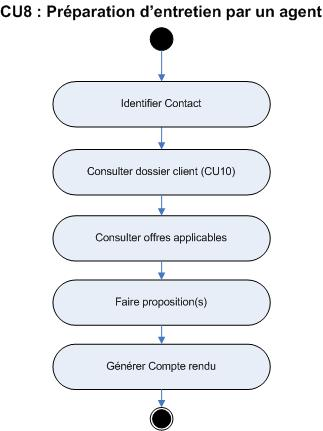
\includegraphics[width=\textwidth]{..\..\diagrammeActivite\DACU8.jpg}
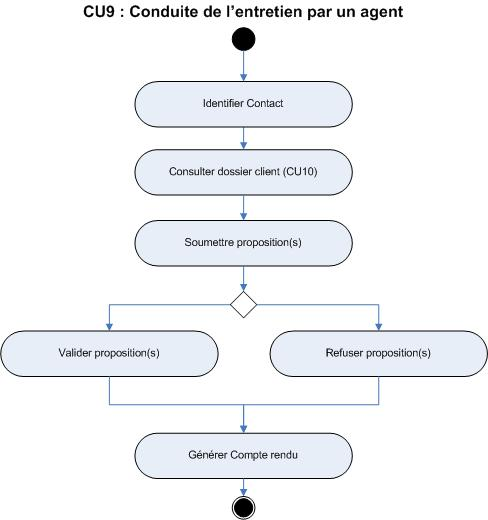
\includegraphics[width=\textwidth]{..\..\diagrammeActivite\DACU9.jpg}
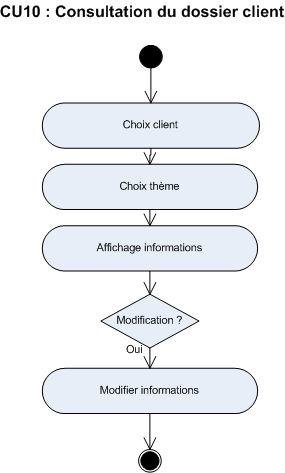
\includegraphics[width=\textwidth]{..\..\diagrammeActivite\DACU10.png}
\end {center}

\subsection{Blocs applicatifs}

\begin {center}
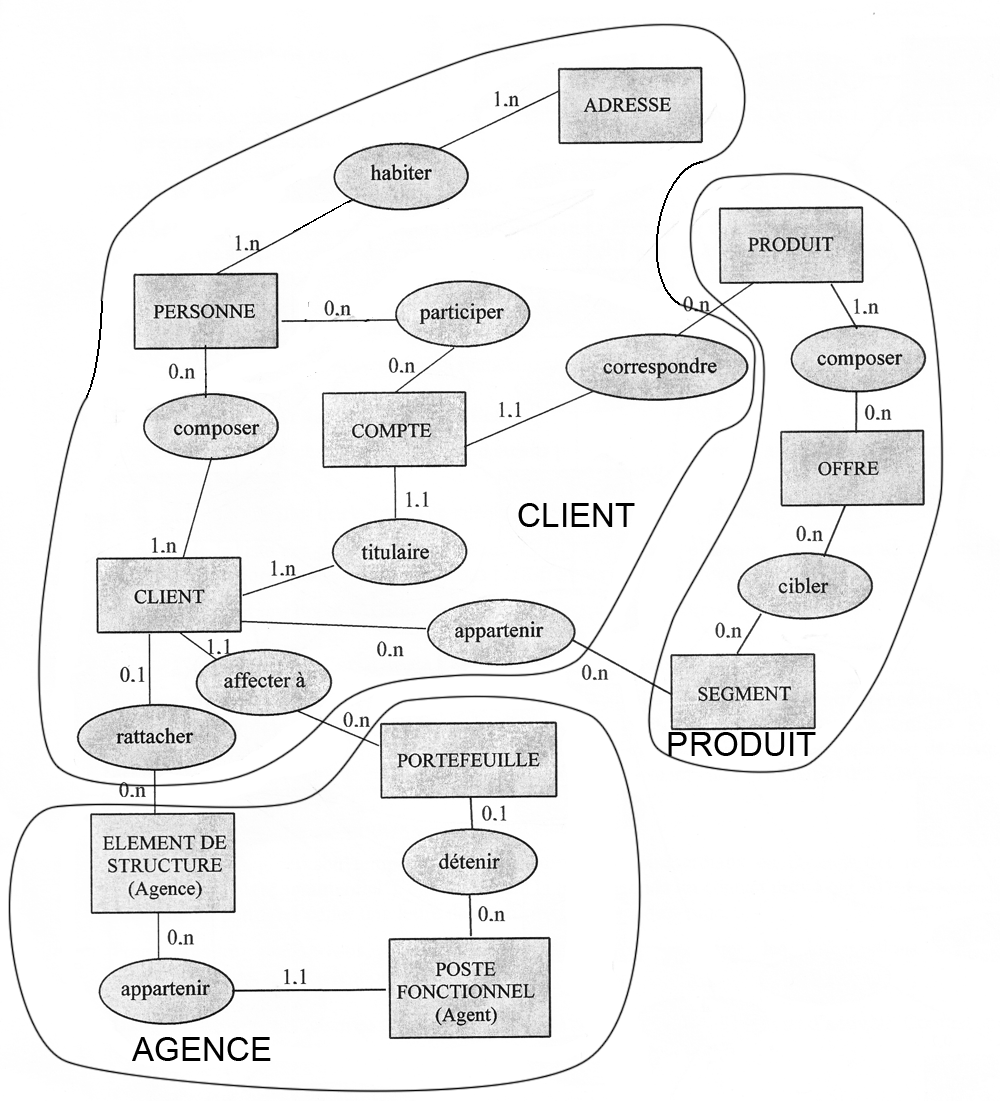
\includegraphics[width=\textwidth]{Decoupage MCD 1.png}
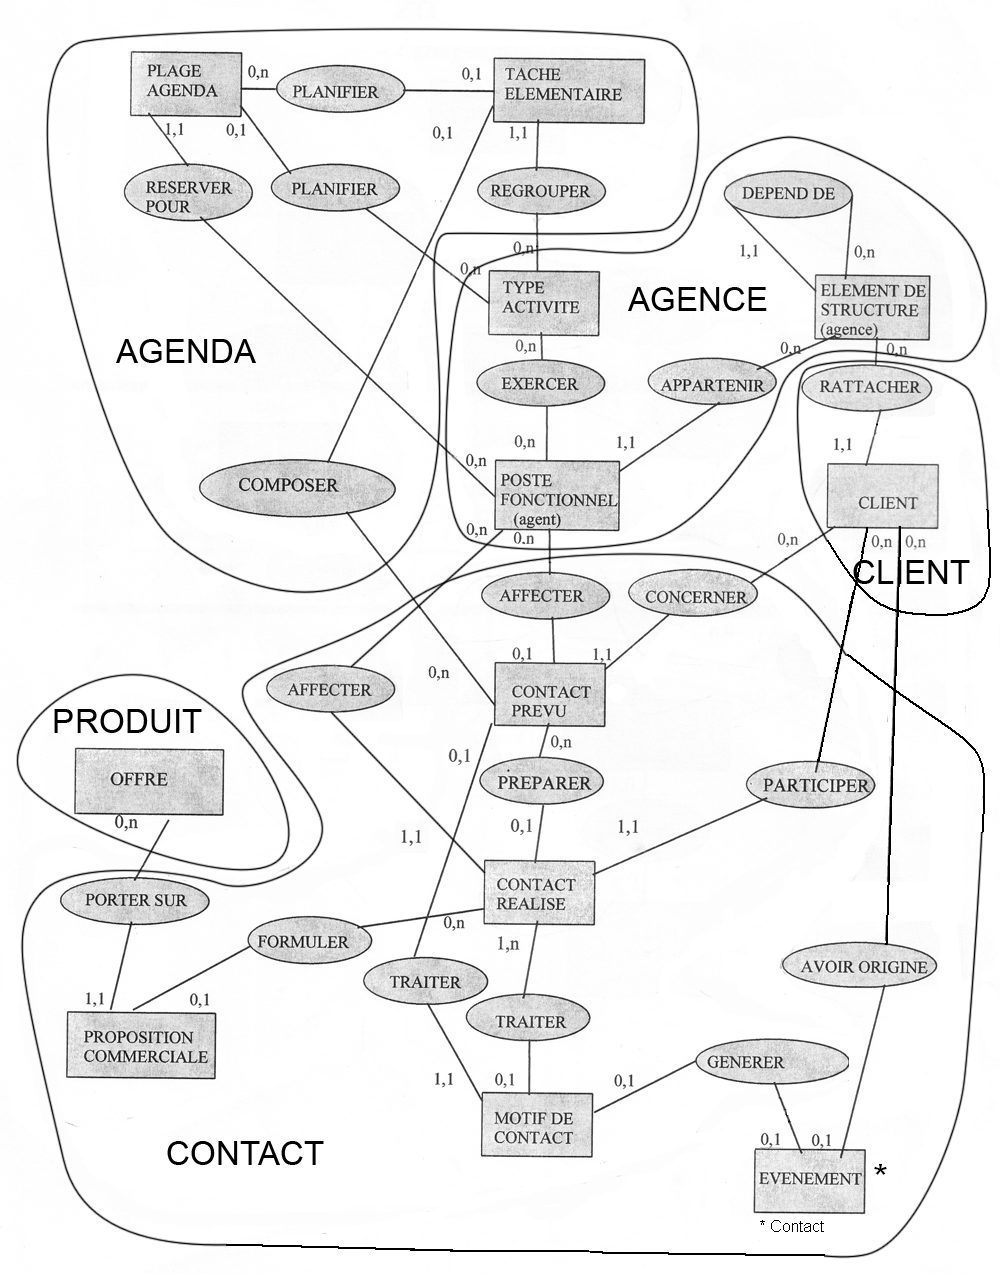
\includegraphics[width=\textwidth]{Decoupage MCD 2.png}
\end {center}

\subsection{Cycles de vie des objets métiers}

Voici le diagramme d'état de l'objet ``Contact'' :

\begin {center}
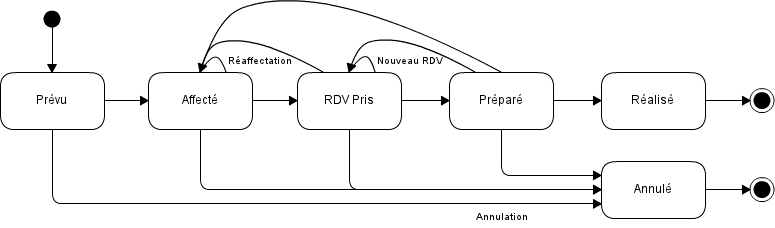
\includegraphics[width=\textwidth]{diagramme-etat-objet-contact.png}
\end {center}
Comme prévu, il n'est pas possible de réaffecter un contact à un autre agent. En effet un agent sera toujours responsable du groupe de contacts qu'on lui a affectés. Néanmoins, les rendez-vous pris, eux, pourront être réaffectés à un autre agent que celui en charge du contact. Cela permettra entre autre de palier à l'absence d'un agent le jour du rendez-vous client.


\subsection{Détermination des flux de l'architecture}

\subsubsection{Diagramme de séquence}

Ci-dessous sont présentés les différents diagrammes de séquences :
\begin {center}
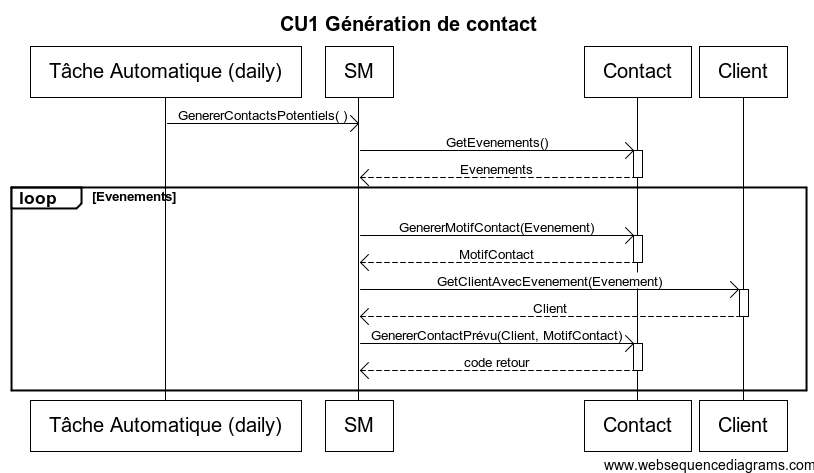
\includegraphics[width=\textwidth]{..\..\webSequenceDiagrameSources\cu1.png}
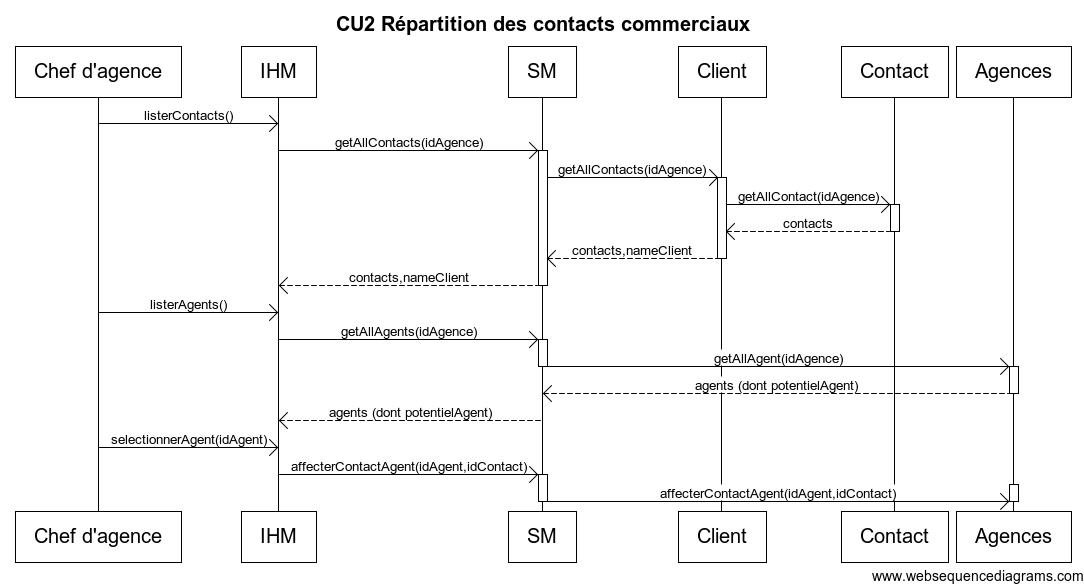
\includegraphics[width=\textwidth]{..\..\webSequenceDiagrameSources\cu2.png}
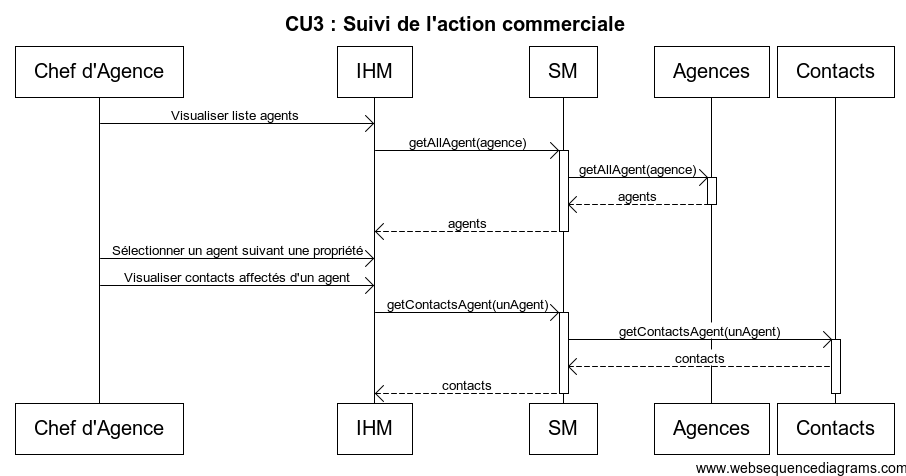
\includegraphics[width=\textwidth]{..\..\webSequenceDiagrameSources\cu3.png}
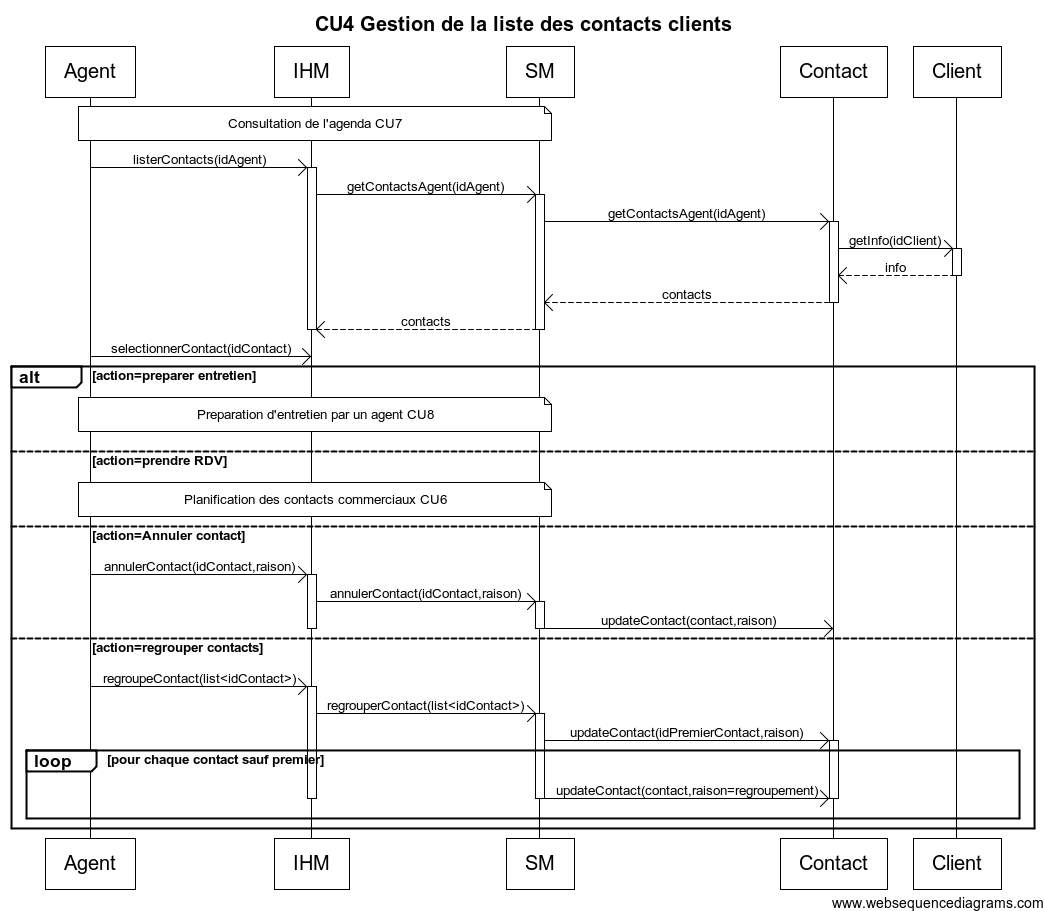
\includegraphics[width=\textwidth]{..\..\webSequenceDiagrameSources\cu4.png}
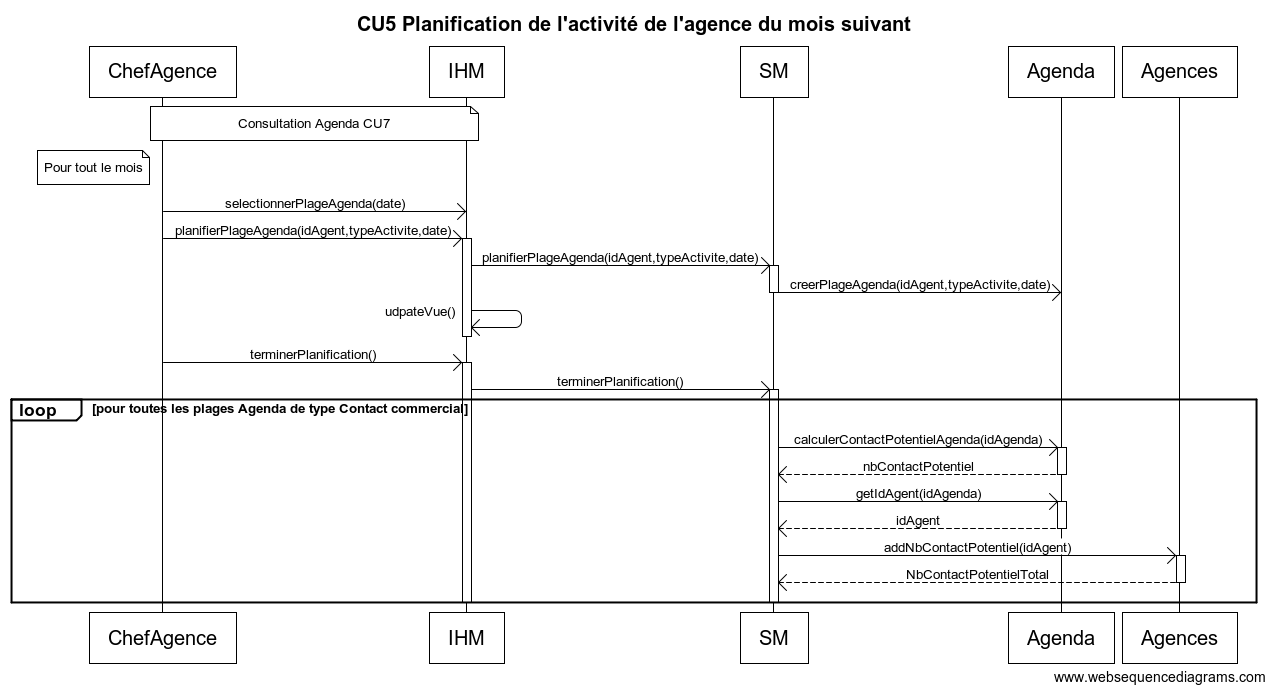
\includegraphics[width=\textwidth]{..\..\webSequenceDiagrameSources\cu5.png}
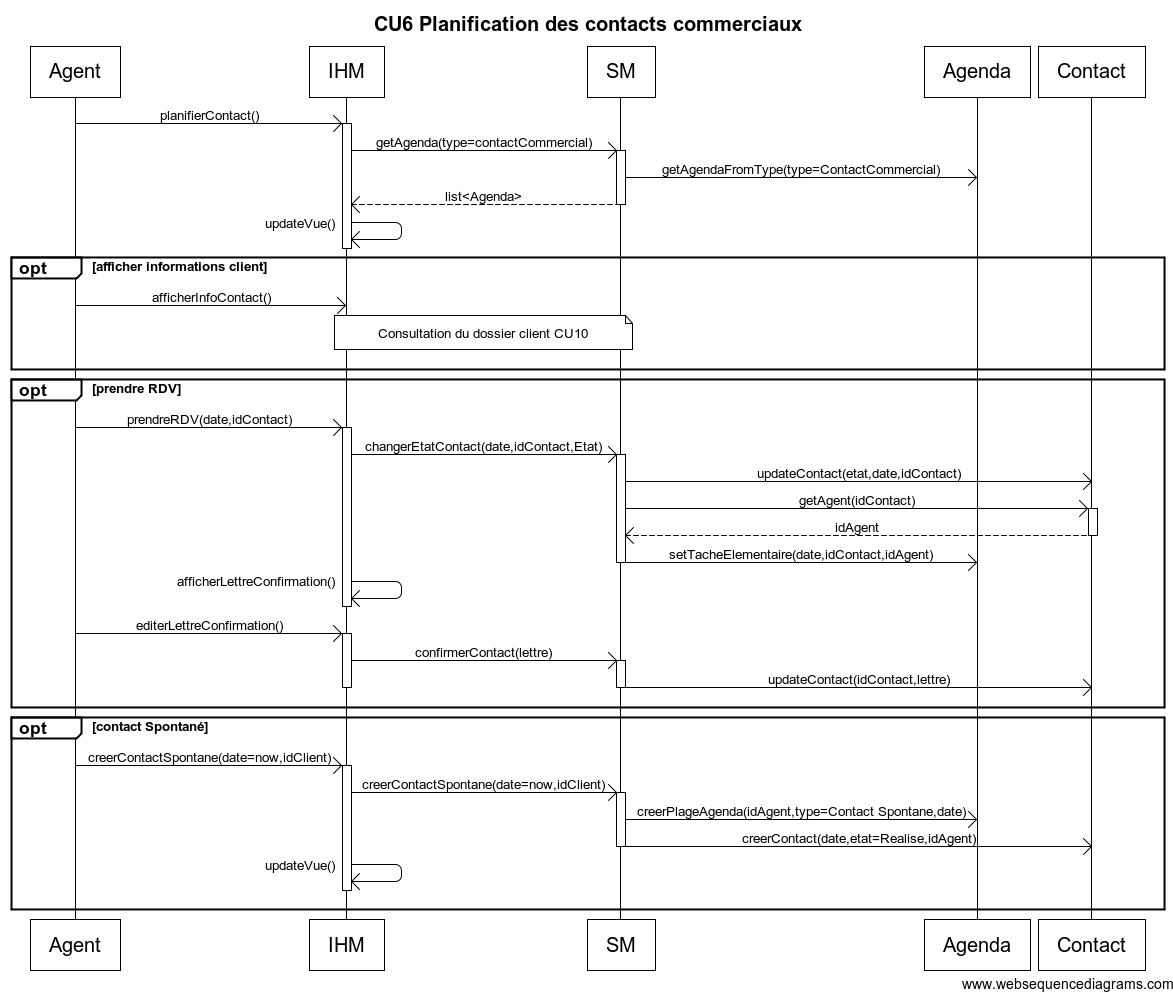
\includegraphics[width=\textwidth]{..\..\webSequenceDiagrameSources\cu6.png}
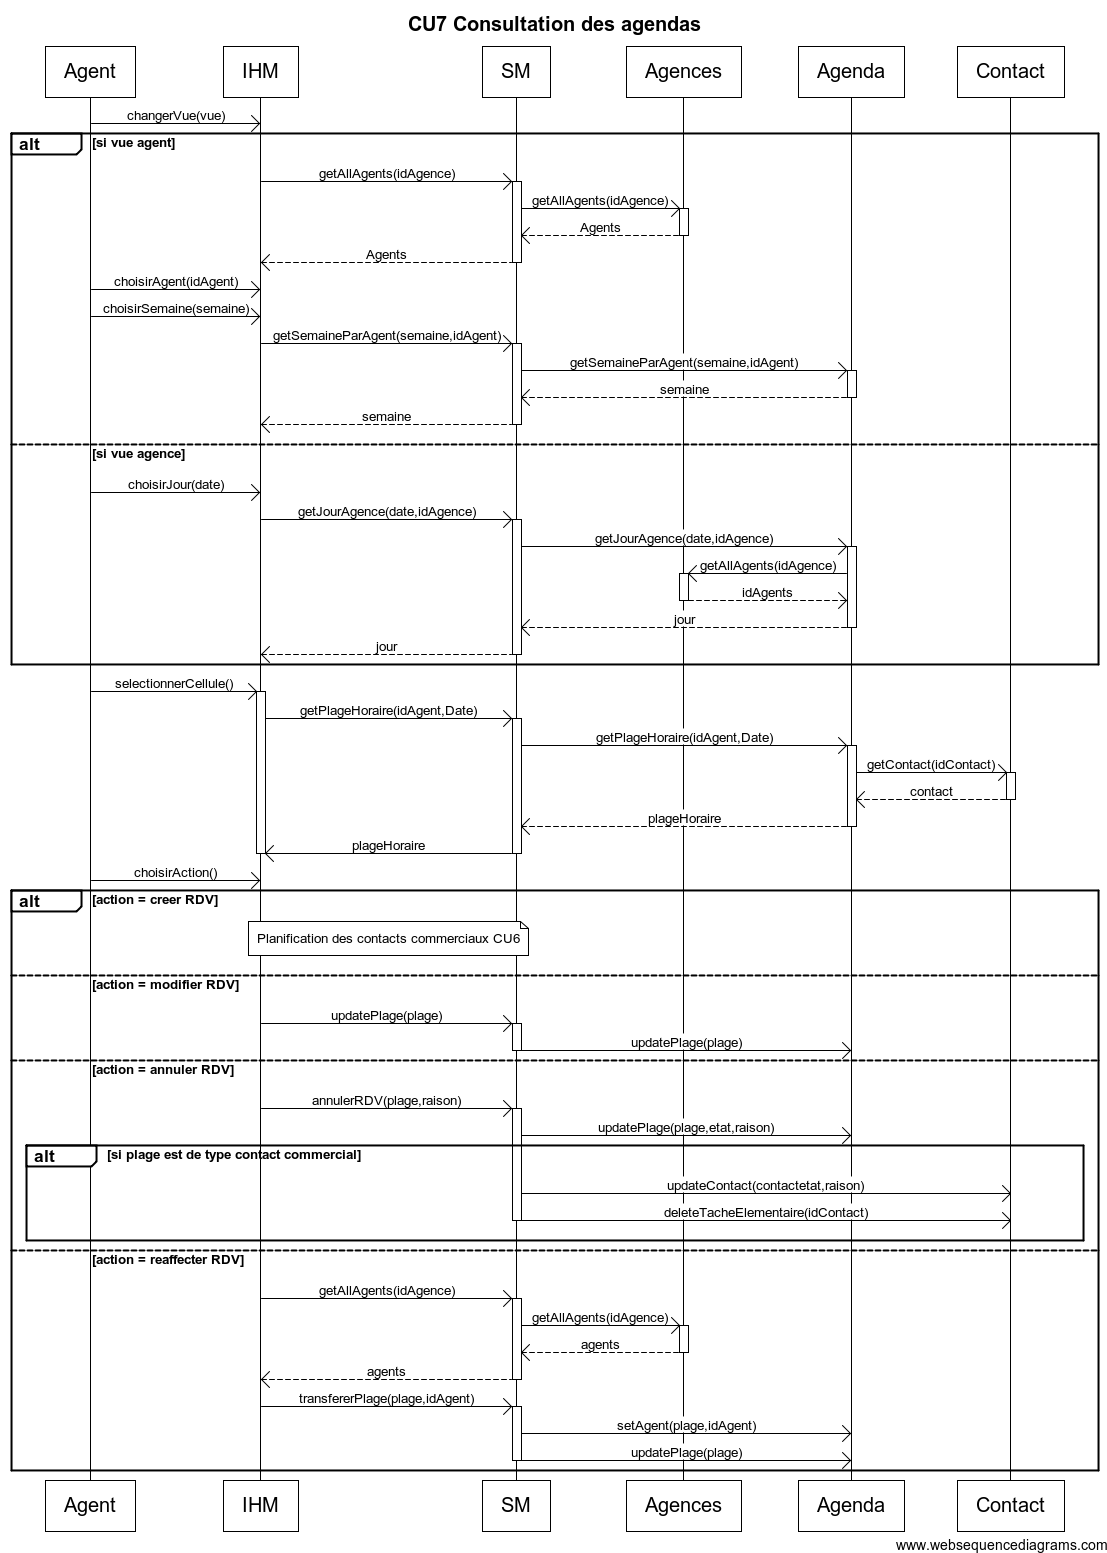
\includegraphics[width=\textwidth]{..\..\webSequenceDiagrameSources\cu7.png}
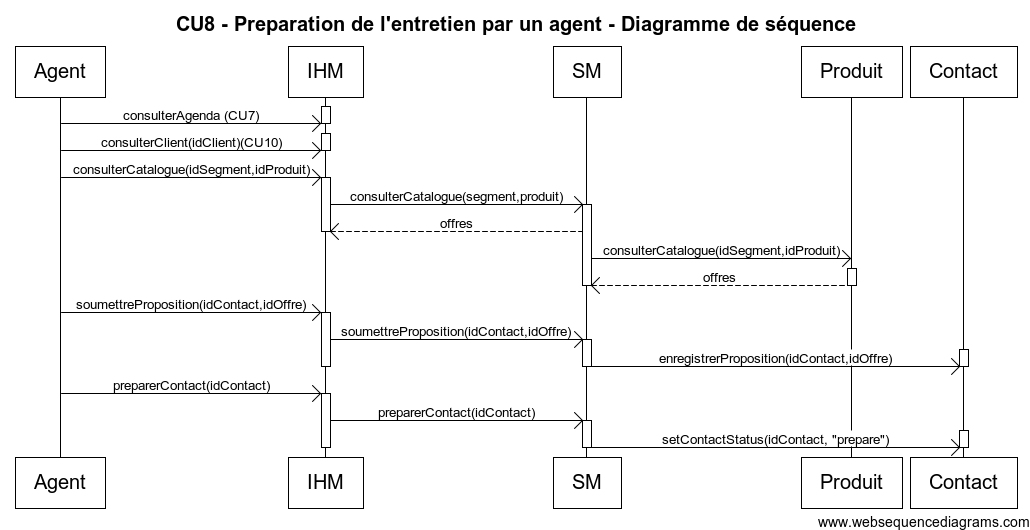
\includegraphics[width=\textwidth]{..\..\webSequenceDiagrameSources\cu8.png}
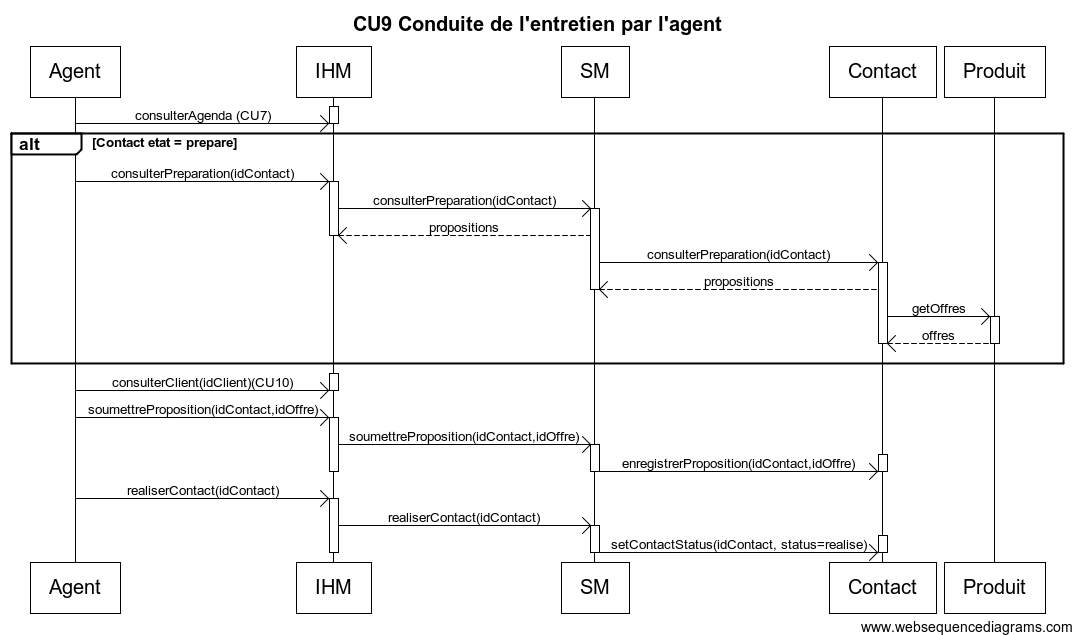
\includegraphics[width=\textwidth]{..\..\webSequenceDiagrameSources\cu9.png}
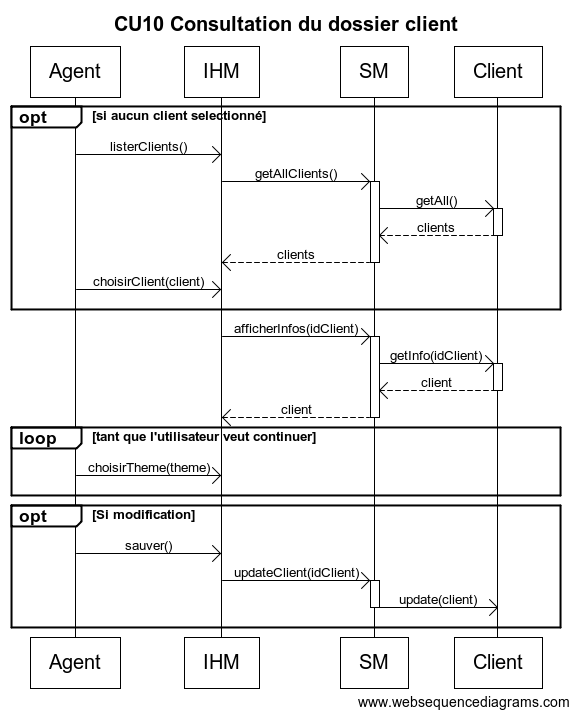
\includegraphics[width=\textwidth]{..\..\webSequenceDiagrameSources\cu10.png}
\end {center}

\subsubsection{Diagramme de collaboration}

Voici le diagramme de collaboration représentatif de la dynamique de
l'architecture:

\begin {center}
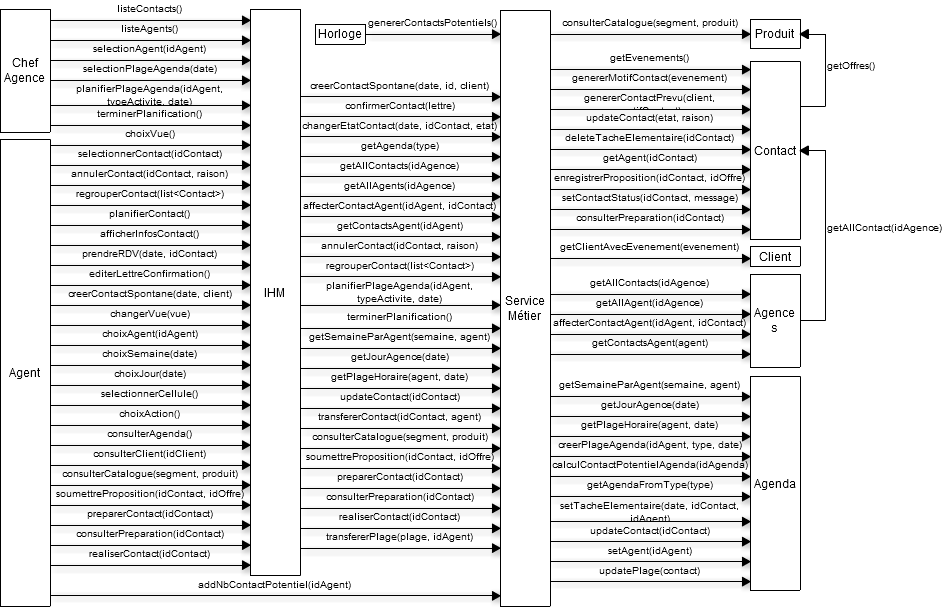
\includegraphics[width=\textwidth]{diagramme-collaboration.png}
\end {center}

Ce diagramme souligne l'existence de flux conséquents entre des groupes de blocs
majeurs, qui permettent d'appuyer le choix de l'architecture retenue, dont nous
discuterons maintenant.


\subsection{Choix de l'environnement technique}
L'environnement technique sera une architecture C/S 3-tiers : l'architecture du système sera donc séparée en trois couches distinctes, à savoir :
\begin{itemize}
\item Couche de données : l'information est stockée ici sur la ou les bases de données. Ces informations seront récuperé par la couche applicative
\item Couche applicative : représente le coeur de l'architecture. A chaque demande de la couche de présentation, la couche applicative va effectuer un calcul, appliquer les règles de gestion et au besoin récuperer les informations de la base de données.
\item Couche de présentation : à chaque action de l'utilisateur, cette couche va d'une part transférer l'information créée par l'utilisateur à la couche applicative et d'autre part afficher l'information récupérée et traitée depuis la base de données par les deux couches précédentes.
\end{itemize}
Le détail de ces tiers sera présenté dans le chapitre 'Architecture technique', notamment la localisation et la répartition des données.
